\section{Results}
\label{sec:results}
%
%Table~\ref{tab:loglikelihood} summarizes the results of the
%experiments comparing the eight combinations over the different
%scenarios. The empirical hybridization is denoted as \emph{EMP}, and
%the reduced representation as \emph{Red}.

%\begin{table}
%  \caption{Log Likelihood Values for each scenario and
%    combination. Higher values correspond to better models. Values in
%    bold are the two highest log likelihood for a scenario. Each value
%    is the average of 10 runs.}
%  \label{tab:loglikelihood}
%  \begin{tabular}{|c|c|c|c|c|c|c|c|c|}
%    \hline
%    & \multicolumn{4}{|c|}{No Pre-processing} & \multicolumn{4}{|c|}{Spectral Clustering}\\
%    Scenario & GA & Red & EMP & EMP-Red & GA & Red & EMP & EMP-Red\\
%    \hline
%    Kanto 2005 & -2291.4 & -2354.1 & -2345.1 & -2557.8 & {\bf-2202.7} & -2233.3 & {\bf-2203.7} & -2355.0\\
%    Kanto 2006 & -2269.2 & -2317.3 & -2350.7 & -2520.0 & {\bf-2173.3} & -2203.1 & {\bf-2175.8} & -2313.5\\
%    Kanto 2007 & -2204.9 & -2235.7 & -2293.3 & -2449.5 & {\bf-2104.1} & -2125.0 & {\bf-2110.3} & -2213.9\\
%    Kanto 2008 & -2203.0 & -2273.2 & -2277.7 & -2501.0 & {\bf-2097.9} & -2124.3 & {\bf-2010.3} & -2245.7\\
%    Kanto 2009 & -2375.6 & -2418.5 & -2463.6 & -2630.7 & {\bf-2279.1} & -2299.1 & {\bf-2282.4} & -2382.0\\
%    Kanto 2010 & -2203.6 & -2296.6 & -2294.9 & -2534.4 & {\bf-2099.5} & -2125.0 & {\bf-2104.0} & -2249.8\\
%    \hline
%    EastJapan 2005 &-2442.8&-2394.9&-2633.6&-2588.4& {\bf-2099.6} & {\bf-2150.2} & -2177.4 & -2300.6 \\
%    EastJapan 2006 &-2211.1&-2191.7&-2408.9&-2390.9&{\bf-1896.7}&{\bf-1960.4}&-1965.7&-2131.8\\
%    EastJapan 2007 &-2112.2&-2100.5&-2305.1&-2294.9&{\bf-1821.9}&{\bf-1889.4}&-1914.4&-2070.0\\
%    EastJapan 2008 &-4139.7&-4288.6&-4301.3&-4424.8&{\bf-3942.5}&{\bf-3989.1}&-4034.9&-4156.8\\
%    EastJapan 2009 &-2281.2&-2221.2&-2498.9&-2416.5&{\bf-1948.5}&{\bf-1087.4}&-2043.7&-2164.5\\
%    EastJapan 2010 &-2577.7&-2579.1&-2783.9&-2783.9&{\bf-2232.7}&{\bf-2291.3}&-2296.9&-2455.2\\
%    \hline
%    %Kansai 2005 & & & & & & & & \\
%    %Kansai 2006 & & & & & & & & \\
%    %Kansai 2007 & & & & & & & & \\
%    %Kansai 2008 & & & & & & & & \\
%    %Kansai 2009 & & & & & & & & \\
%    %Kansai 2010 & & & & & & & & \\
%    %\hline
%    %Tohoku 2005 & & & & & & & & \\
%    %Tohoku 2006 & & & & & & & & \\
%    %Tohoku 2007 & & & & & & & & \\
%    %Tohoku 2008 & & & & & & & & \\
%    %Tohoku 2009 & & & & & & & & \\
%    %Tohoku 2010 & & & & & & & & \\
%    %\hline
%  \end{tabular}
%\end{table}

%% ANOVA ANALYSIS
%
%To better understand these results, we performed an ANOVA analysis
%over all log-likelihoods obtained from the 8 combinations, paired by
%year and region. The resulting F-value was 18.9, indicating that there
%is an effect associated with the combinations.
%
%To identify where is this effect, we perform a one versus all Dunnet
%test ($\alpha = 0.05$), using GAModel as the base. The confidence
%intervals obtained from the test can be seen on
%Figure~\ref{fig:Dunnet}.
%
%\begin{figure}
%  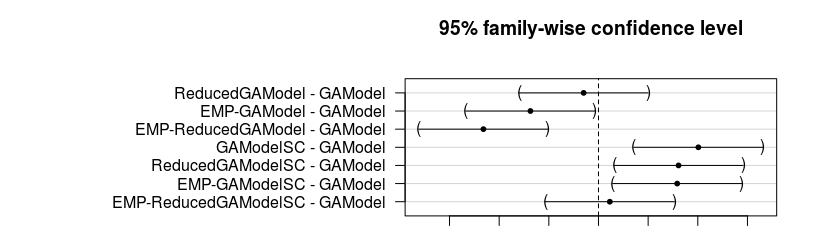
\includegraphics[width=1\textwidth]{img/dunnet}
%  \caption{Conf. Intervals of the difference between GAModel and each combination.}
%  \label{fig:Dunnet}
%\end{figure}
%
%%% HEAT MAP
%
%To get a better intuition about what these results mean in concrete
%terms, we show one example of a set of risk models generated by the
%proposed variations in Figure~\ref{fig:heatmap}.
%
%\begin{figure}
%\centering
%\begin{subfigure}{.5\textwidth}
%  \centering
%  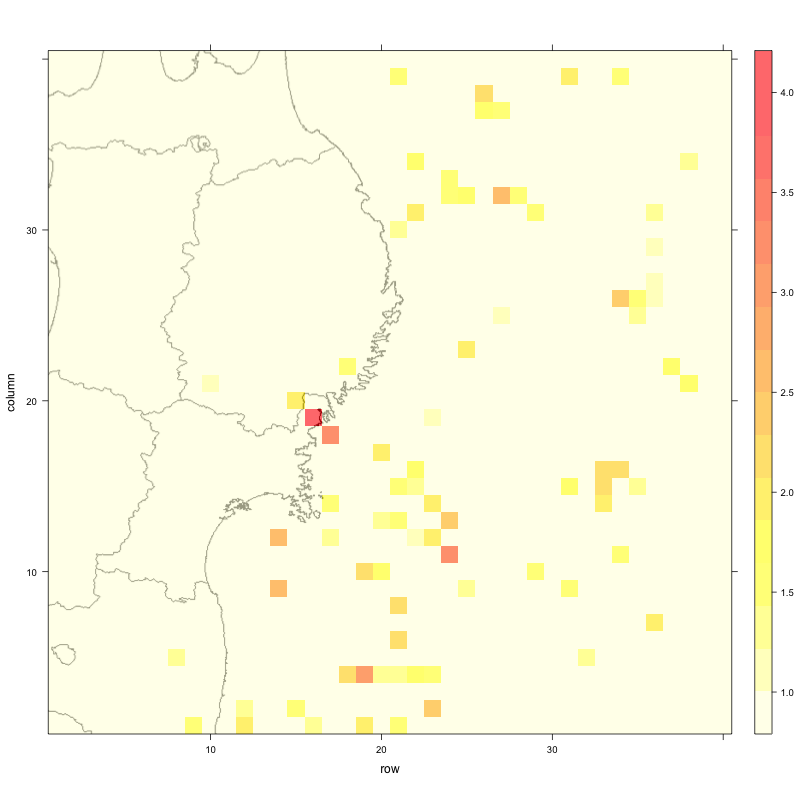
\includegraphics[width=1\linewidth]{img/gaModel}
%  \caption{GAModel}
%  \label{fig:sub1}
%\end{subfigure}%
%\begin{subfigure}{.5\textwidth}
%  \centering
%  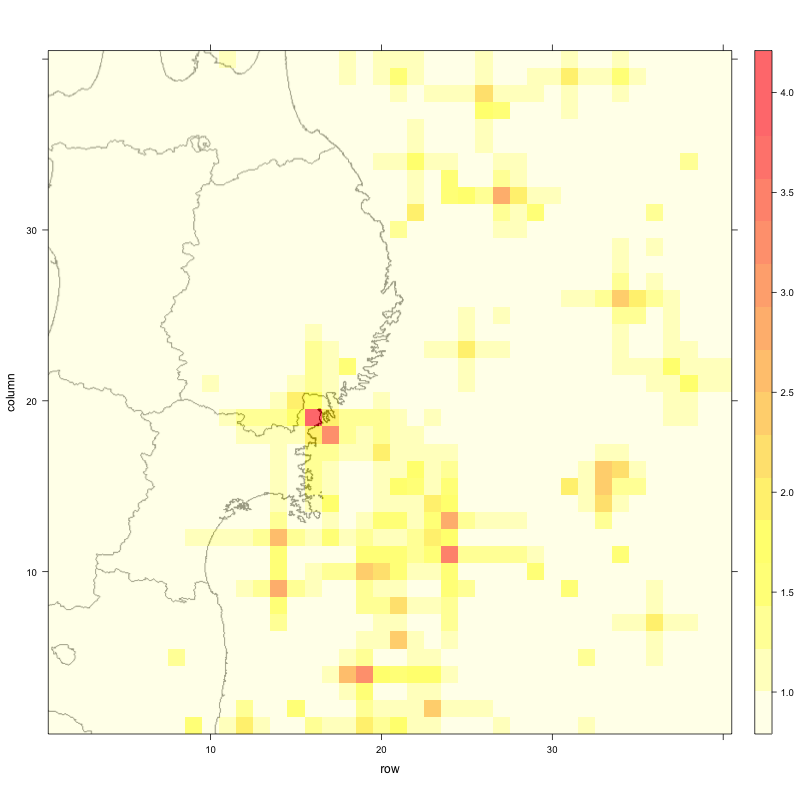
\includegraphics[width=1\linewidth]{img/SC-EMP-ga}
%  \caption{Spectral Clustering with Emp-GA}
%  \label{fig:sub2}
%\end{subfigure}\\
%\begin{subfigure}{.5\textwidth}
%  \centering
%  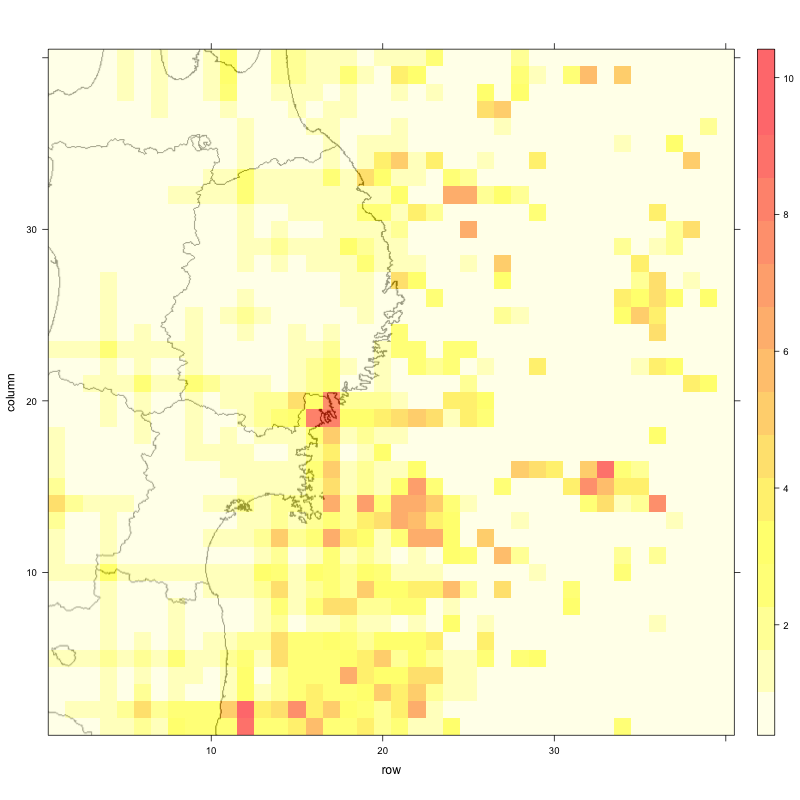
\includegraphics[width=1\linewidth]{img/EMP-RED-ga}
%  \caption{EMP-GA with Reduced Representation}
%  \label{fig:sub3}
%\end{subfigure}%
%\begin{subfigure}{.5\textwidth}
%  \centering
%  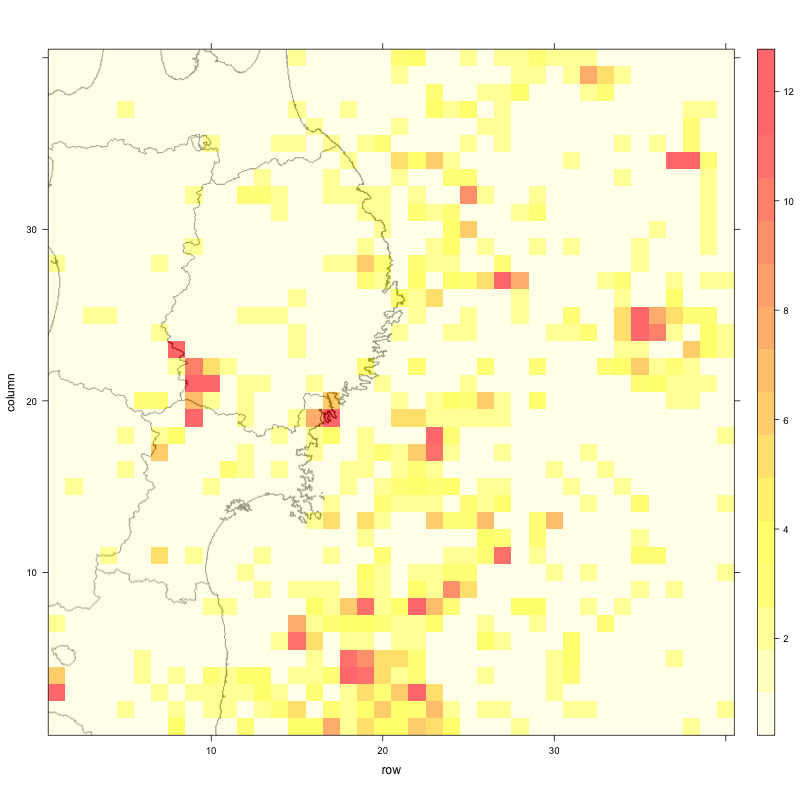
\includegraphics[width=1\linewidth]{img/realEastJapan_2010}
%  \caption{Earthquake Catalog}
%  \label{fig:sub4}
%\end{subfigure}
%\caption{Earthquake Risk Model heat maps, for scenario East Japan
%  2010. Darker colors correspond to higher number of earthquakes}
%\label{fig:heatmap}
%\end{figure}
%
